%%%%%%%%%%%%%%%%%%%%%%%%%%%%% Define Article %%%%%%%%%%%%%%%%%%%%%%%%%%%%%%%%%%
\documentclass{article}
%%%%%%%%%%%%%%%%%%%%%%%%%%%%%%%%%%%%%%%%%%%%%%%%%%%%%%%%%%%%%%%%%%%%%%%%%%%%%%%

%%%%%%%%%%%%%%%%%%%%%%%%%%%%% Using Packages %%%%%%%%%%%%%%%%%%%%%%%%%%%%%%%%%%
\usepackage{listings, xcolor}
\usepackage{parskip}
\usepackage{hyperref}
\usepackage{amsmath}
\usepackage{graphicx}
\usepackage[a4paper, margin = 1.5cm]{geometry}
\usepackage{float}
\usepackage{amsmath}
\usepackage{amssymb}
\usepackage{parskip}
\usepackage{listings}

\lstset{
frame = shadowbox,
basicstyle = \small\ttfamily,
mathescape = true,
numbers = left,
commentstyle = \itshape\color{gray}
columns = flexible,
keepspaces = true,
moredelim = [l]{//}
}

%%%%%%%%%%%%%%%%%%%%%%%%%%%%%% Title & Author %%%%%%%%%%%%%%%%%%%%%%%%%%%%%%%%
\title{Statechart}
\author{Trentin Tommaso}
%%%%%%%%%%%%%%%%%%%%%%%%%%%%%%%%%%%%%%%%%%%%%%%%%%%%%%%%%%%%%%%%%%%%%%%%%%%%%%
\begin{document}
\maketitle
\tableofcontents
\newpage

  \section{Notazzioni}
    \subsection{Macchina a stati}
      Macchina caratterizzata da tre elementi fondamentali (stati, eventi, transizioni): la macchina può esistere in un numero finito di \textbf{stati} e, in risposta a \textbf{eventi}, eseguire \textbf{transizioni} tra gli stati.
    \subsection{Stato}
      Condizione della vita di un'entità durante la quale essa può:
      \begin{itemize}
          \item Soddisfare una condizione;
          \item Eseguire un'attività;
          \item Aspettare un evento.
      \end{itemize}
      In un dato istante l'entità si può trovare in uno e un solo stato, in un certo stato essa si comporterà in uno specifico modo in risposta a eventi specifici.
    \subsection{Evento}
      Occorrenza di interesse, collocata nel tempo e nello spazio, che può scatenare il cambiamento di stato dell'entità. Il comportamento della stessa entità di fronte agli eventi può cambiare se si trova in stati diversi.
    \subsection{Transizione di stato}
      Passaggio da uno stato all'altro, in risposta a un evento, etichettato con la sintassi \textbf{evento trigger[guardia]/attività}:
      \begin{itemize}
          \item \textbf{evento trigger} è l'evento (o sequenza di eventi) che scatena la transizione, può contenere parametri;
          \item \textbf{guardia} è una condizione booleana che deve essere verificata per il verificarsi della transizione;
          \item \textbf{attività} è un'azione elaborativa che si verifica contestualmente con la transizione.
      \end{itemize}
      \begin{figure}[htpb]
          \centering
          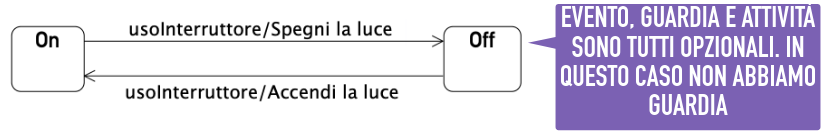
\includegraphics[width=0.7\linewidth]{figures/trans.png}
      \end{figure}
    \subsection{Statechart diagram}
      Grafo diretto in cui i nodi sono gli stati e gli archi sono le transizioni (complessivo di stati speciali quali \textbf{stato iniziale} e \textbf{stato finale}).
      \subsubsection{Eventi con guardie mutualmente esclusive}
        \noindent
          \begin{minipage}[c]{0.58\linewidth}
            \begin{itemize}
               \item Quando sistema si trova in uno stato, un evento può scatenare una sola transizione uscente da quello stato;
               \item Quando sistema si trova in uno stato, lo stesso evento trigger può portare a due stati diversi solo se guardie sono mutualmente esclusive.
            \end{itemize}
          \end{minipage}
        \hfill
          \begin{minipage}[c]{0.38\linewidth}
            \centering
              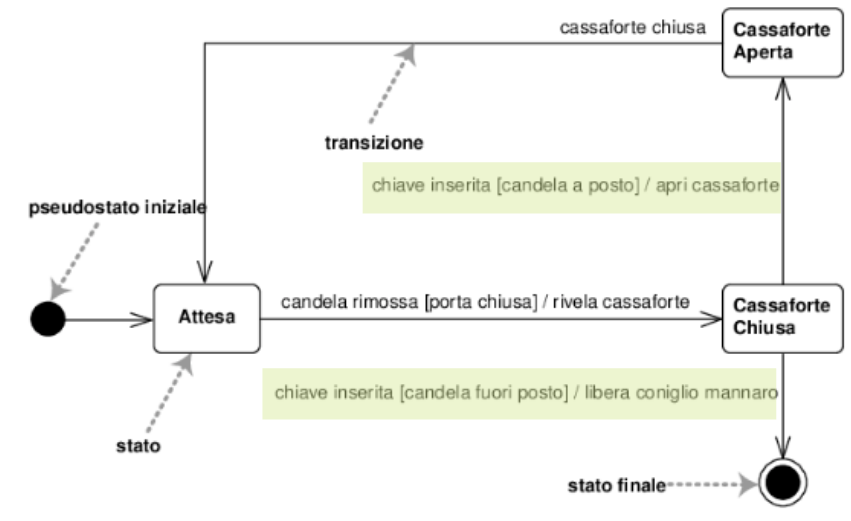
\includegraphics[width=0.8\linewidth]{figures/statechart_gme.png}
          \end{minipage}
      \subsubsection{Eventi che non scatenano transizioni}
        \noindent
          \begin{minipage}[c]{0.58\linewidth}
              \begin{itemize}
                  \item Se in uno stato si verifica un evento per cui non esistono transizioni valide, quell'evento viene ignorato;
                  \item Es. se sistema si trova in stato Cassaforte chiusa, eventi di cassaforte chiusa e candela rimossa non causano transizioni.
              \end{itemize}
          \end{minipage}
          \hfill
          \begin{minipage}[c]{0.38\linewidth}
              \centering
              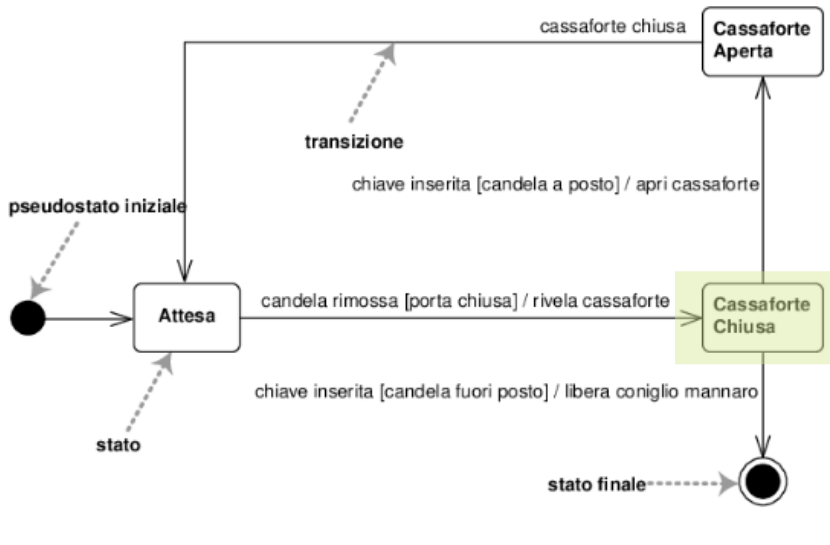
\includegraphics[width=0.8\linewidth]{figures/statechart_enst.png}
          \end{minipage}
      \subsubsection{Stato finale / transizione}
        \noindent
          \begin{minipage}[c]{0.58\linewidth}
              \begin{itemize}
                  \item Stato finale indica completamento dell'esecuzione della macchina a stati;
                  \item Solitamente passaggio a stato finale sottintende distruzione dell'oggetto;
                  \item Bisogna ricreare oggetto per ritornare allo stato iniziale.
              \end{itemize}
          \end{minipage}
          \hfill
          \begin{minipage}[c]{0.38\linewidth}
              \centering
              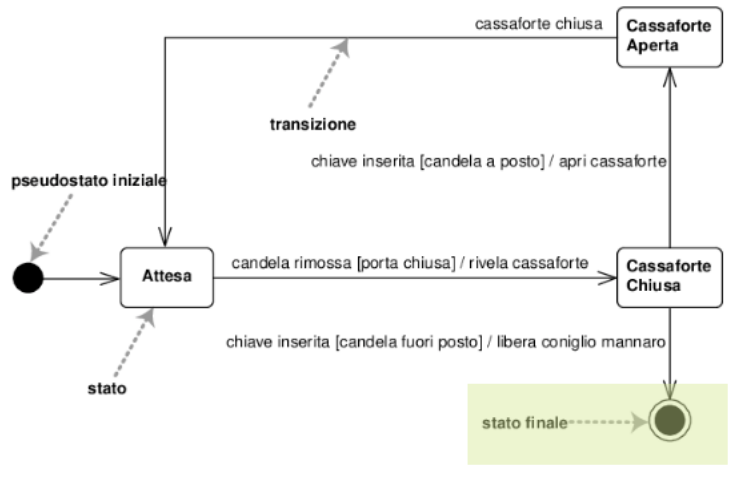
\includegraphics[width=0.8\linewidth]{figures/statechart_sf.png}
          \end{minipage}
      \subsubsection{Esempio statechart diagram}
        \begin{figure}[htpb]
          \centering
            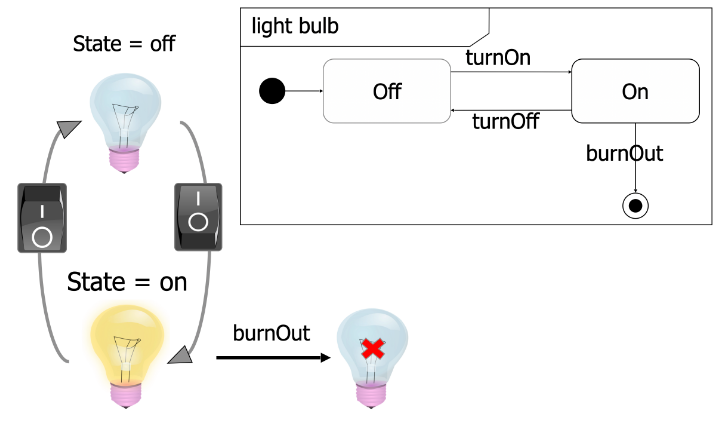
\includegraphics[width=0.7\linewidth]{figures/statechart_es.png}
        \end{figure}
  \section{Attività interne}
    Risposte ad eventi che conducono a stesso stato possono essere indicate come \textbf{auto-transizioni} o \textbf{attività interne}, in queste attività interne uno stato risponde a eventi senza eseguire transizione a un'altro stato, ma scatenando attività interne (evento, guardia e attività vengono riportate nel box dello stato).
    \begin{figure}[htpb]
        \centering
        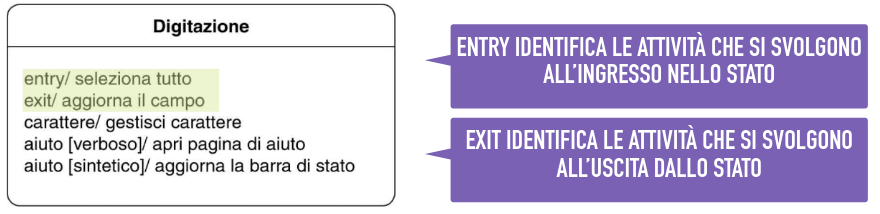
\includegraphics[width=0.7\linewidth]{figures/att_int.png}
    \end{figure}
    La differenza tra \textit{auto-transizioni} e \textit{attività-interne} è che nelle ultime non avvienee il nuovo ingresso nello stato (non vengono quindi rieseguite le attività di \textit{entry} e \textit{exit}).
    \begin{figure}[htpb]
        \centering
        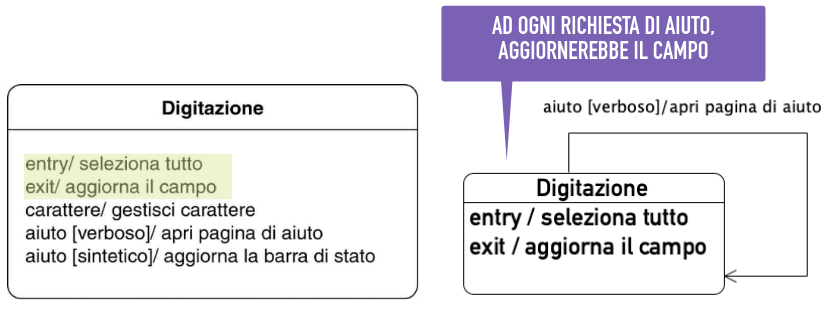
\includegraphics[width=0.7\linewidth]{figures/att_int_diff.png}
    \end{figure}
    \subsection{Activity state}
      Stati in cui l'oggetto svolge determinata attività in modo continuato invece di essere in attesa inerte di un evento per agire, le \textbf{do-activity} sono attività interne particolari svolte da entità mentre si trova nello stato.
      \begin{figure}[htpb]
          \centering
          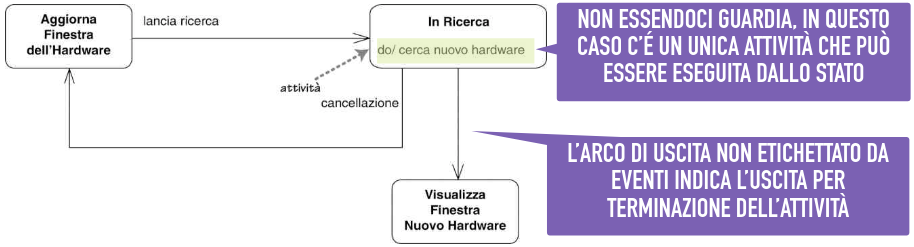
\includegraphics[width=0.7\linewidth]{figures/do_act.png}
      \end{figure}
      Le do-activity hanno durata temporale finita e possono essere interrotte, mentre le attività regolari sono istantanee ed atomiche, non influenzate / interrotte da altri eventi.
  \section{Superstati}
    \subsection{Annidamento}
      Strato composto: annidamento (\textit{nesting}) di stati permette di dettagliare comportemento interno di uno stato mediante sottostati.
    \subsection{Superstati}
      Stati composti che contengono un intero statechart diagram (gli stati del diagramma contenuto sono chiamati sottostati). I sottostati possono condividere certe transizioni / attività interne, mentre il superstato raccoglie il comportamento dei suoi sottostati.
      \begin{figure}[htpb]
          \centering
          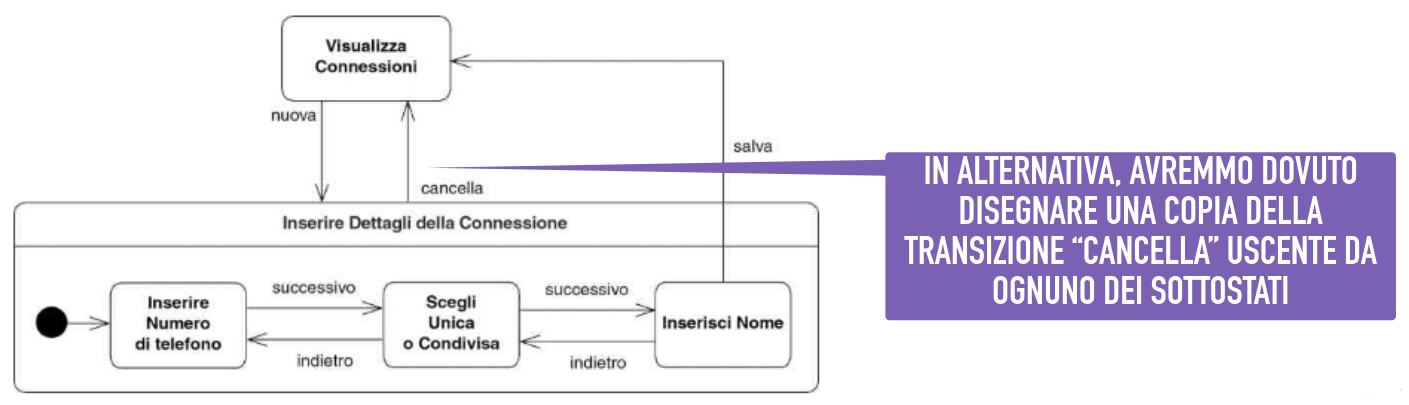
\includegraphics[width=0.7\linewidth]{figures/superstati_1.png}
      \end{figure}
      Quando gli archi sono diretti verso il superstato, in generale si intende che sono diretti verso il so stato iniziale di default.
      \begin{figure}[htpb]
          \centering
          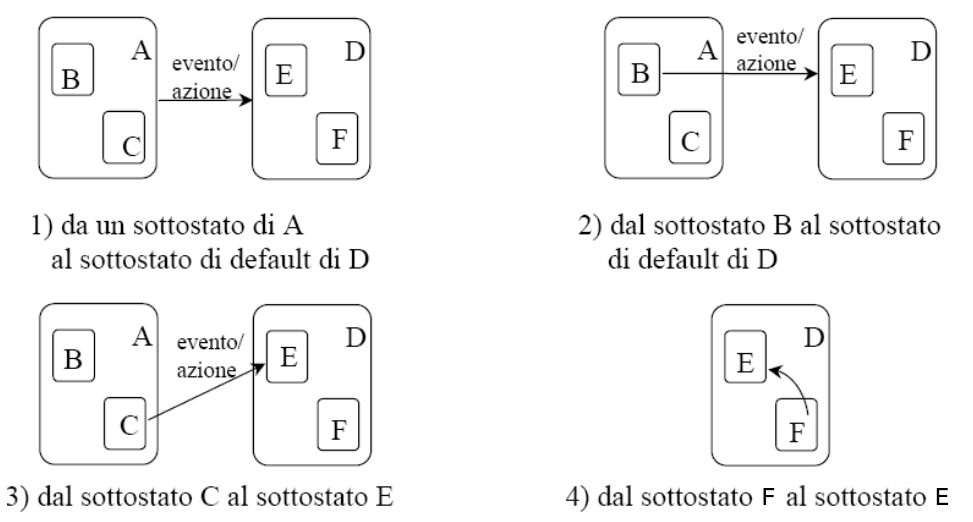
\includegraphics[width=0.8\linewidth]{figures/superstati_2.png}
      \end{figure}
  \section{Stati concorrenti}
    \noindent
      \begin{minipage}[c]{0.58\linewidth}
          Uno stato può essere diviso (mediante linee tratteggiate interne al superstato) in regioni che contengono sottostati da eseguire in modo concorrente.
      \end{minipage}
      \hfill
      \begin{minipage}[c]{0.38\linewidth}
          \centering
          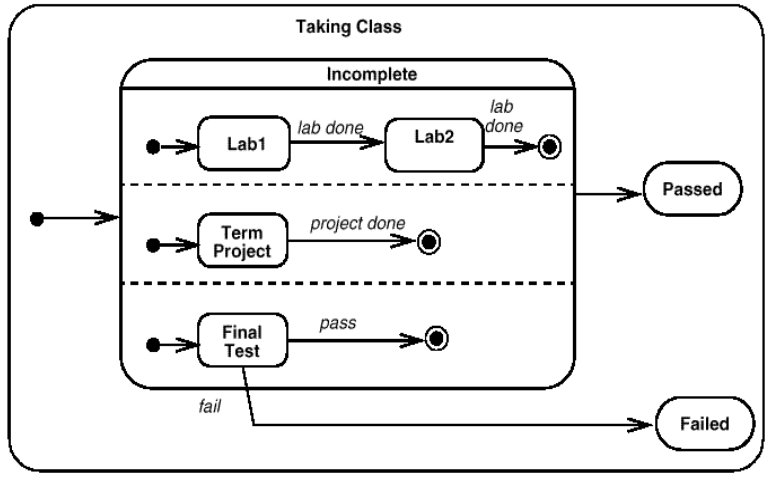
\includegraphics[width=0.8\linewidth]{figures/stat_con.png}
      \end{minipage}
  \section{Implementazione}
    Uno statechart (a livello di dettaglio) può essere implementato in tre modi principali:
    \begin{itemize}
        \item utilizzando una catena di switch nidificati;
        \item applicando Pattern State;
        \item utilizzando tabelle di stato.
    \end{itemize}
    \subsection{Statechart da implementare}
      \begin{figure}[htpb]
          \centering
          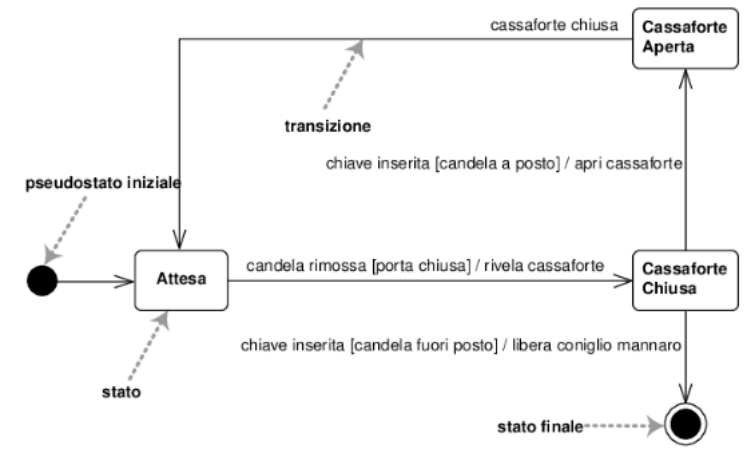
\includegraphics[width=0.6\linewidth]{figures/sc_impl_1.png}
      \end{figure}
    \subsection{Implementazione switch nidificati}
      \noindent
        \begin{minipage}[c]{0.58\linewidth}
            \begin{itemize}
                \item \textbf{Vantaggi}
                  \begin{itemize}
                      \item Soluzione più intuitiva.
                  \end{itemize}
                \item Svantaggi
                  \begin{itemize}
                      \item Implementazione complessa (codice complesso anche per casi semplici);
                      \item Necessità di gestire modifiche apportate in più punti del codice.
                  \end{itemize}
            \end{itemize}
        \end{minipage}
        \hfill
        \begin{minipage}[c]{0.38\linewidth}
            \centering
            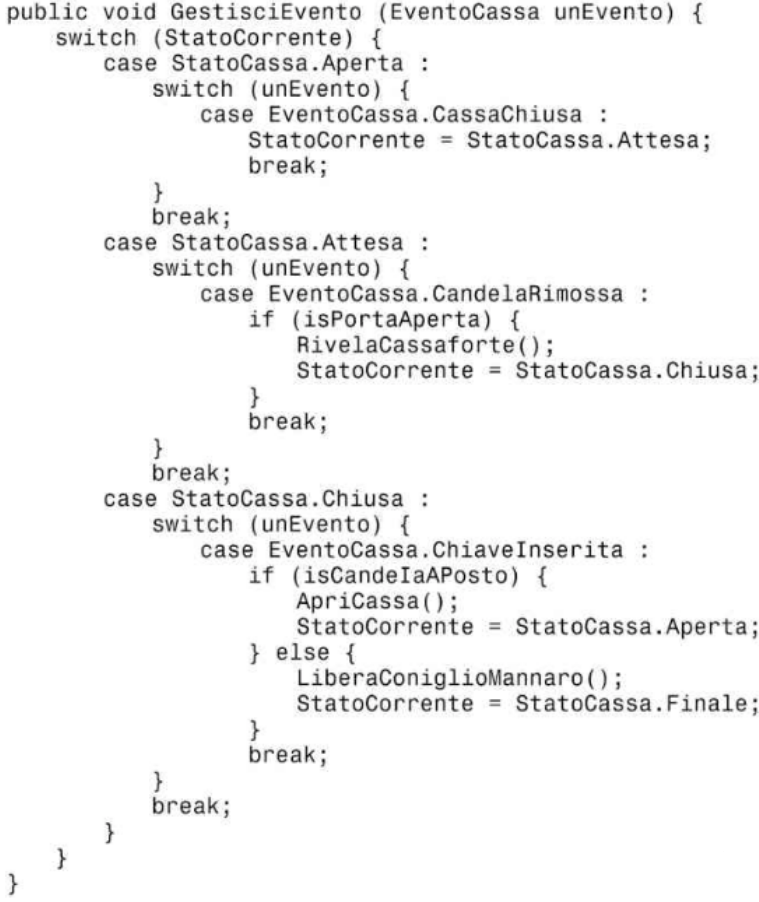
\includegraphics[width=0.8\linewidth]{figures/sc_impl_2.png}
        \end{minipage}
    \subsection{Implementazione pattern state}
      \noindent
        \begin{minipage}[c]{0.48\linewidth}
            Statechart viene tradotto con:
            \begin{itemize}
                \item Classe \textbf{controller} che mantiene traccia dello stato corrente e implementa medoto di cambiamento di stato / si limita a inoltrare chiamate a classi stato;
                \item Classe \textbf{di stato} che dichiara metodi corrispondenti a ogni evento e li implementa in modo che non facciano nulla;
                \item Classi \textbf{stato derivate} corrispondenti agli stati del programma, implementano soltanto metodi corrispondenti a eventi scatenabili su quello stato per overriding.
            \end{itemize}
        \end{minipage}
        \hfill
        \begin{minipage}[c]{0.48\linewidth}
            \centering
            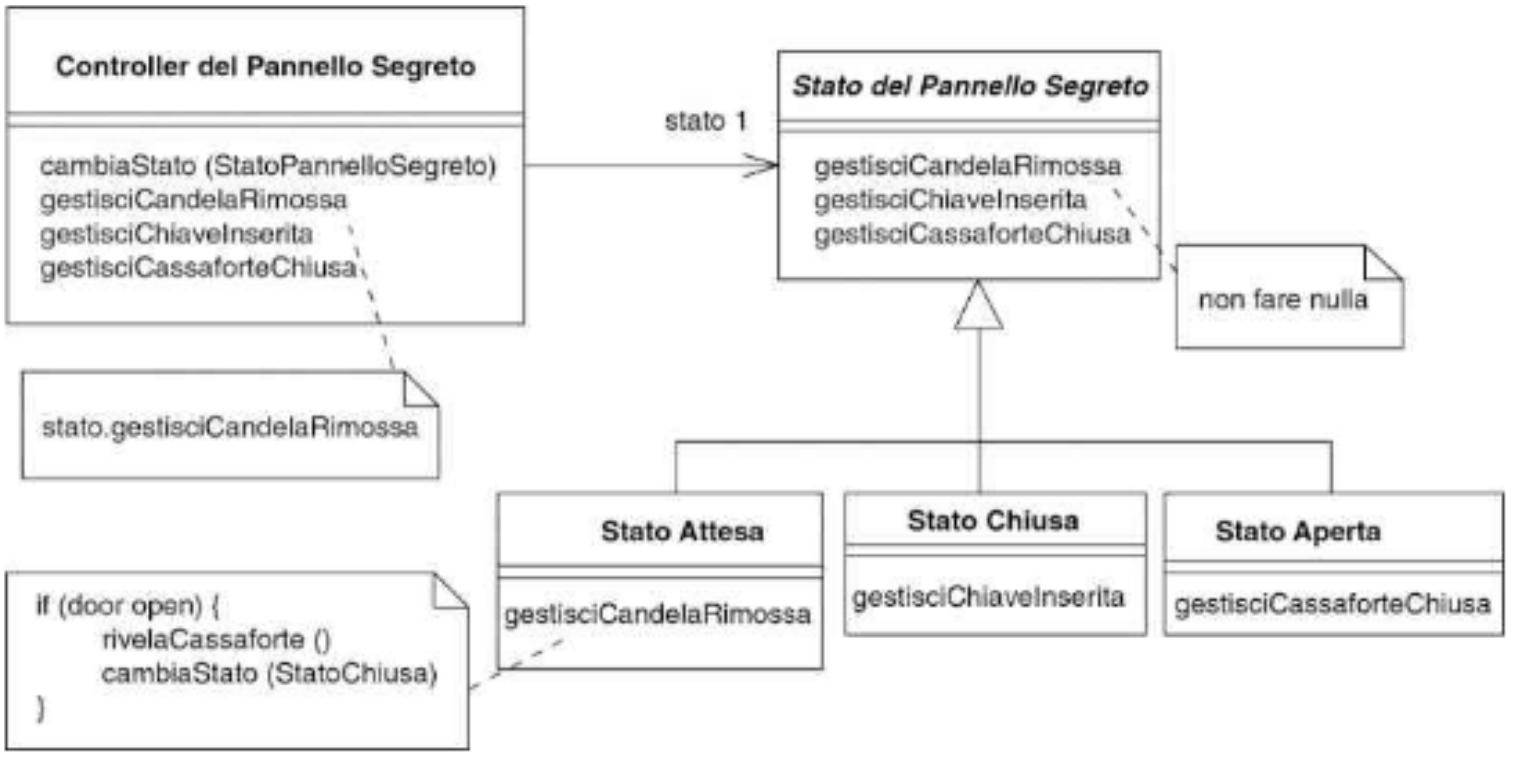
\includegraphics[width=\linewidth]{figures/sc_impl_3.png}
        \end{minipage}
    \subsection{Implementazione tabelle di stato}
      Rappresentazione tabellare delle informazioni contenute nel diagramma, tabella direttamente interpretata a runtime da apposito interprete oppure trasformata in codice da strumenti di generazioen automatica del codice.
      \begin{figure}[htpb]
          \centering
          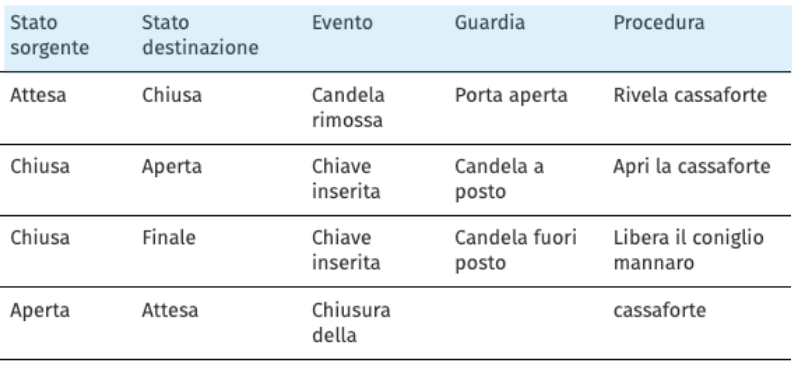
\includegraphics[width=0.7\linewidth]{figures/sc_impl_4.png}
      \end{figure}
  \section{Conclusioni - Applicabilità}
    \begin{itemize}
        \item \textbf{Vantaggi}
          \begin{itemize}
              \item Diagrammi di stato servono a descrivere comportamento di un oggetto in più casi d'uso;
              \item Utili a rappresentare classi con logiche interne complesse / particolarmente interessanti.
          \end{itemize}
        \item \textbf{Svantaggi}
          \begin{itemize}
              \item Non molto utili a descriere collaborazioni tra oggetti (per questo scopo sono preferibili Sequence / Activity diagram);
              \item Loro implementazione corrisponde a codice ripetitivo, quindi si usano spesso generatori automatici di codice.
          \end{itemize}
    \end{itemize}
\end{document}
